%! Tex program = pdflatex
 
\documentclass[UTF8]{ctexart}
\CTEXsetup[format={\Large\bfseries}]{section}
\usepackage{amsmath}
\usepackage{ctex}
\usepackage{array}
\usepackage{ulem}
\usepackage{graphicx}
\usepackage{geometry}
\usepackage{multirow}
\usepackage{subfig}
\usepackage{float}
\usepackage{multicol}
\usepackage{multirow}
\usepackage{indentfirst}
\usepackage{makecell}
\geometry{papersize={21cm,29.7cm}}
\geometry{left=2.54cm,right=2.54cm,top=3.18cm,bottom=3.18cm}
\usepackage{fancyhdr}
\pagestyle{fancy}
\lhead{\today}
\chead{}
\rhead{2020011075}
\lfoot{清华大学}
\cfoot{\thepage}
\rfoot{物理实验B(2)}
\renewcommand{\headrulewidth}{0.4pt}
\renewcommand{\headwidth}{\textwidth}
\renewcommand{\footrulewidth}{0pt}
\usepackage{bm}
\begin{document}
\begin{titlepage}
    \begin{center}
		\quad \\
		\quad \\
        \quad \\
        \quad \\
        \quad \\
        \quad \\
		\kaishu \fontsize{30}{15} 逸出功的测量
	\end{center}
	\vskip 10cm

    \begin{center}
        \begin{large}
        \begin{tabular}{cc}
        院\qquad 系:& ~~~~~~~~自动化系~~~~~~~~      \\
        \cline{2-2}\\
        班\qquad 级:& 自02班   \\
        \cline{2-2}\\
        学生姓名:& 彭程    \\
        \cline{2-2}\\
        学\qquad 号:&2020011075   \\
        \cline{2-2}\\
        组\qquad 号:& 双四下L    \\
        \cline{2-2}\\
        座~~位~~号:& \# 5    \\
        \cline{2-2}
        \end{tabular}
        \end{large}
        \end{center}

\end{titlepage}
\newpage
\tableofcontents
\newpage
\section{实验名称}
逸出功的测量

\section{数据处理}

\subsection{实验线路图}

\begin{figure}[H]
  \centering
  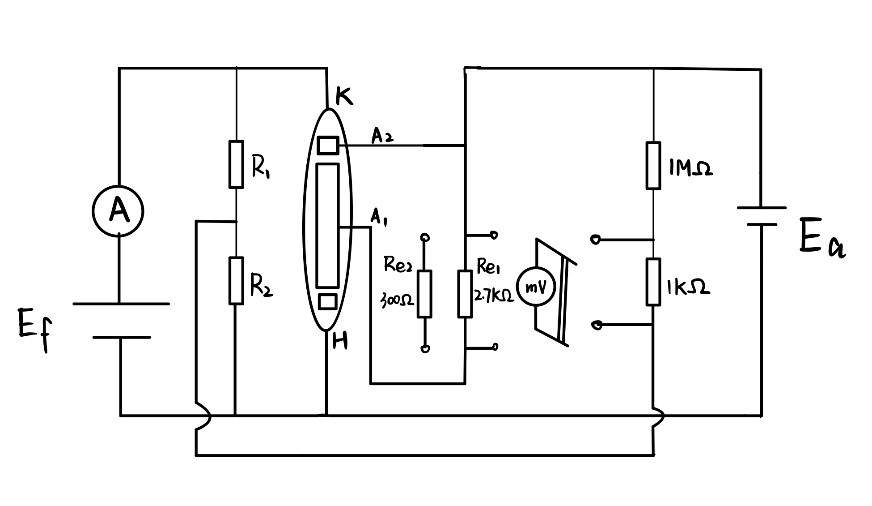
\includegraphics[scale=1]{电路图.jpg}
\end{figure}


\subsection{测量数据记录}

\begin{tabular}{c|c|c|c|c|c|c|c|c|c}
  \hline 倍率  & $I_{f}(A) T(K)$ &$ U_{a} U_{e}^{\prime}$ & 1 & 2 & 3 & 4 & 5 & 6 & 7 \\
  \hline \multirow{2}{*}{$\times 1$} & $0.500 \mathrm{~A}$ & $U_{a}(V)$ & 36.01 & 49.02 & 63.99 & 81.00 & 100.03 & 121.03 & 144.00 \\
  \cline { 2 - 10 } & 1726.0 K & $U_{e}^{\prime}(mV) $& 3.20 & 3.28 & 3.37 & 3.44 & 3.51 & 3.60 & 3.68 \\
  \hline \multirow{2}{*}{$\times 1$} & $0.540 \mathrm{~A}$ & $U_{a}(V)$ & 36.02 & 48.98 & 64.00 & 80.99 & 100.03 & 120.99 & 144.00 \\
  \cline { 2 - 10 } & 1792.4 K & $U_{e}^{\prime}(mV)$ & 11.15 & 11.39 & 11.64 & 11.89 & 12.14 & 12.41 & 12.66 \\
  \hline \multirow{2}{*}{$\times 1$} & $0.580 \mathrm{~A}$ & $U_{a}(V)$ & 35.98 & 49.02 & 64.01 & 81.01 & 99.99 & 121.01 & 144.00 \\
  \cline { 2 - 10 } & 1864.2 K & $U_{e}^{\prime}(mV)$ & 34.84 & 35.63 & 36.39 & 37.13 & 37.86 & 38.66 & 39.44 \\
  \hline \multirow{2}{*}{$\times 1$} & $0.620 \mathrm{~A}$ & $U_{a}(V)$ & 36.04 & 48.98 & 63.99 & 80.98 & 100.02 & 121.04 & 144.01 \\
  \cline { 2 - 10 } & 1930.6 K & $U_{e}^{\prime}(mV)$ & 97.70 & 99.79 & 101.93 & 104.00 & 105.95 & 108.01 & 110.10 \\
  \hline \multirow{2}{*}{$\times 10$} & $0.660 \mathrm{~A}$ & $U_{a}(V)$ & 35.98 & 49.03 & 63.99 & 80.97 & 100.04 & 121.03 & 144.02 \\
  \cline { 2 - 10 } & $1991.8 \mathrm{~K}$ & $U_{e}^{\prime}(mV)$ & 26.69 & 27.23 & 27.75 & 28.27 & 28.78 & 29.31 & 29.85 \\
  \hline \multirow{2}{*}{$\times 10$} & $0.700 \mathrm{~A}$ & $U_{a}(V)$ & 36.01 & 49.02 & 64.02 & 80.99 & 99.99 & 121.02 & 144.02 \\
  \cline { 2 - 10 } & 2059.0 K & $U_{e}^{\prime}(mV)$ & 62.39 & 63.60 & 64.80 & 65.98 & 67.10 & 68.35 & 69.54 \\
  \hline
  \end{tabular}

\subsection{温度T的测量}

温度 $ T (/ K)  $的计算方法为对 $ I_{f} \sim T$  关系表进行线性插值所得:
以 $ I_{f}=0.540 \mathrm{~A} $ 为例, 查表可知,  $I_{f}=0.500 \mathrm{~A}$  时,  T=1726 K ; $I_{f}=0.550 \mathrm{~A}$  时,  $T=1809 \mathrm{~K} $ 。因而,  $I_{f}=0.541 \mathrm{~A} $ 时, 灯丝温度的计算公式为:
$$
T=\frac{(0.541-0.500) \times (1809-1726)}{0.550-0.500}+1726=1792.4 \mathrm{~K}
$$

同理可计算出实验中加热电流对应的温度为:\\
\begin{center}
  \begin{tabular}{c|c|c|c|c|c|c}
    \hline 加热电流(A)  & 0.500&0.540&0.580&0.620&0.660&0.700 \\
    \hline 温度(K)  & 1726.0&1792.4&1864.2&1930.6&1991.8&2059.0 \\
    \hline
  \end{tabular}
\end{center}


\subsection{里查孙直线法确定逸出电位和逸出功}

首先就实验手册中的思考问题进行讨论,即若本实验中$R_e$ 未给出具体数值,能否根据$U'_e$和 T 求出逸出电位$\varphi$:

\begin{equation}
  \lg \frac{I_{e}}{T^{2}}=\lg AS-5.039 \times 10^{3} \frac{\varphi}{T}\tag*{(1)}
\end{equation}

\begin{equation}
  \lg I_{e}^{\prime}=\lg I_{e}+\frac{4.39}{2.303 T} \frac{1}{\sqrt{r_{1} \ln \left(r_{2} / r_{1}\right)}} \sqrt{U_{a}}\tag*{(2)}
\end{equation}

由于  $I_{e}^{\prime}$  与  $U_{e}^{\prime}$  满足  $I_{e}^{\prime}=\frac{U_{e}^{\prime}}{R}$ , 其中  $R=2.7 k \Omega$  或  $R=270 k \Omega$  。将此关系式代入式 (2) 可得:

$$
\lg U_{e}^{\prime}=\lg I_{e} R+\frac{4.39}{2.303 T} \frac{1}{\sqrt{r_{1} \ln \left(r_{2} / r_{1}\right)}} \sqrt{U_{a}}
$$

因此, 数据处理时可以直接利用  $U_{e}^{\prime}$  进行直线拟合, 所得截距的物理含义为 $ \lg I_{e} R$ , 不妨记为  $\lg U_{e}$  。

同时由于式(1)可以变形成:
$$
\lg \frac{I_{e} R}{T^{2}}=\lg A S R-5.039 \times 10^{3} \frac{\varphi}{T} 
$$

代入$\lg U_{e}= \lg I_{e}R$ ,有:


\begin{equation}
  \lg \frac{U_{e}}{T^{2}} =\lg A S R-5.039 \times 10^{3} \frac{\varphi}{T} \tag*{(3)}
\end{equation}

因此, 可以利用所得直线截距  $\lg U_{e}$  得到 $ \lg \frac{u_{e}}{T^{2}} $ 并直接进行线性拟合, 同样可求得  $\varphi $ 的值。这样做可 以避免对$  I_{e} $ 的值进行计算。事实上, 由于电阻  R  的值并非精确的 $ 2.7 k \Omega$  或  $300 \Omega$ , 直接计算得到的$  I_{e}$  可 能并非准确值, 这样可以避免产生实验误差。

首先根据实验数据绘制不同温度(加热电流)下$\lg U_{e}'-\sqrt{U_{a}} $的图像:
\begin{figure}[H]
  \centering
  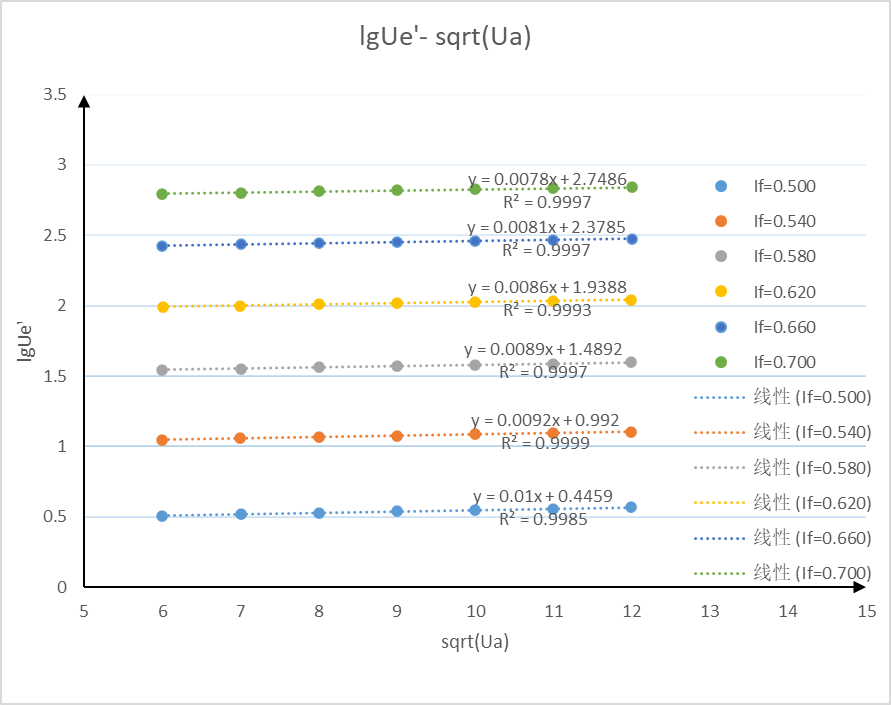
\includegraphics[scale=0.9]{图1.png}
\end{figure}

注意到图中相关系数均大于0.99,表明具有良好的线性性。


从图中获得的截距,即$\lg U_{e}= \lg I_{e}R$的值及相关数据如下表:

\begin{center}
  \begin{tabular}{c|c|c|c|c|c|c}
    \hline 加热电流 (A) & 0.500&0.540&0.580&0.620&0.660&0.700 \\
    \hline 温度(K)  & 1726.0&1792.4&1864.2&1930.6&1991.8&2059.0 \\
    \hline $\lg U_{e}$  & 0.4459&0.9920&1.4892&1.9388&2.3785&2.7486 \\
    \hline $\lg \frac{U_{e}}{T^2}$  &-6.0282&-5.5149&-5.0518&-4.6326&-4.2200&-3.8787 \\
    \hline
  \end{tabular}
\end{center}

根据数据拟合$\lg \frac{U_{e}}{T^2}-\frac{1}{T}$ 的图像:
\begin{figure}[H]
  \centering
  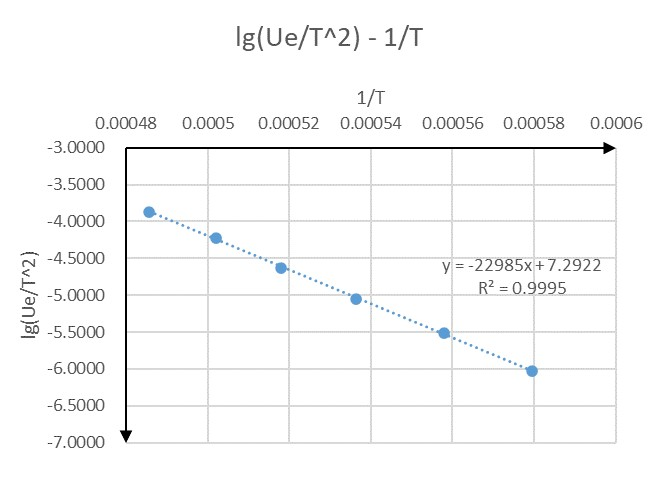
\includegraphics[scale=0.9]{图2.jpg}
\end{figure}
注意到图中相关系数为0.9995,表明线性相关。

由式(3)可知,该直线斜率应为$-5.039 \times 10^{3} \varphi$,故:
$$
\varphi=\frac{-22985}{-5.039 \times 10^{3}}=4.56V
$$

溢出功为:
$$
W_0=e_0\varphi=4.56eV
$$

测量值与理论值4.54eV的相对偏差为:
$$
\delta=\frac{4.56-4.54}{4.56}\times 100\% =0.44\%
$$
\section{实验总结}

本实验在预习计算与设计上涉及到较多的电路原理相关知识,考验了我们对于之前的物理知识掌握的细致程度,为了很好的保证预习质量与实验正确性,在预习过程中我复习了电学相关知识,使我的电学基础知识得到了进一步的巩固。

在实际操作上有一定的复杂度,涉及到较多线路的接线以及两个电路的混合联接,且工作电压差距较大。在接线过程中,需要谨慎细致的操作,保证了一遍接线成功,避免对仪器造成损坏。

在数据处理部分考验使用现代计算工具的熟练使用,在使用excel绘制实验数据表格与处理数据的过程中,我深切的体会到了现代绘图工具的简便快捷。

本实验中让我最有收获的应当是公式变形从而减少不必要参数测量的思想,通过里查孙直线法避免了A、S的测量,通过$lg U_e'$和$\sqrt{U_a}$的线性关系避免了$I_e$的计算。这些巧妙的数学变形对我以后的学习有了很大的触动。

最后,感谢老师对我们的悉心指导!

\section{原始数据及预习思考题}

\begin{figure}[H]
  \centering
  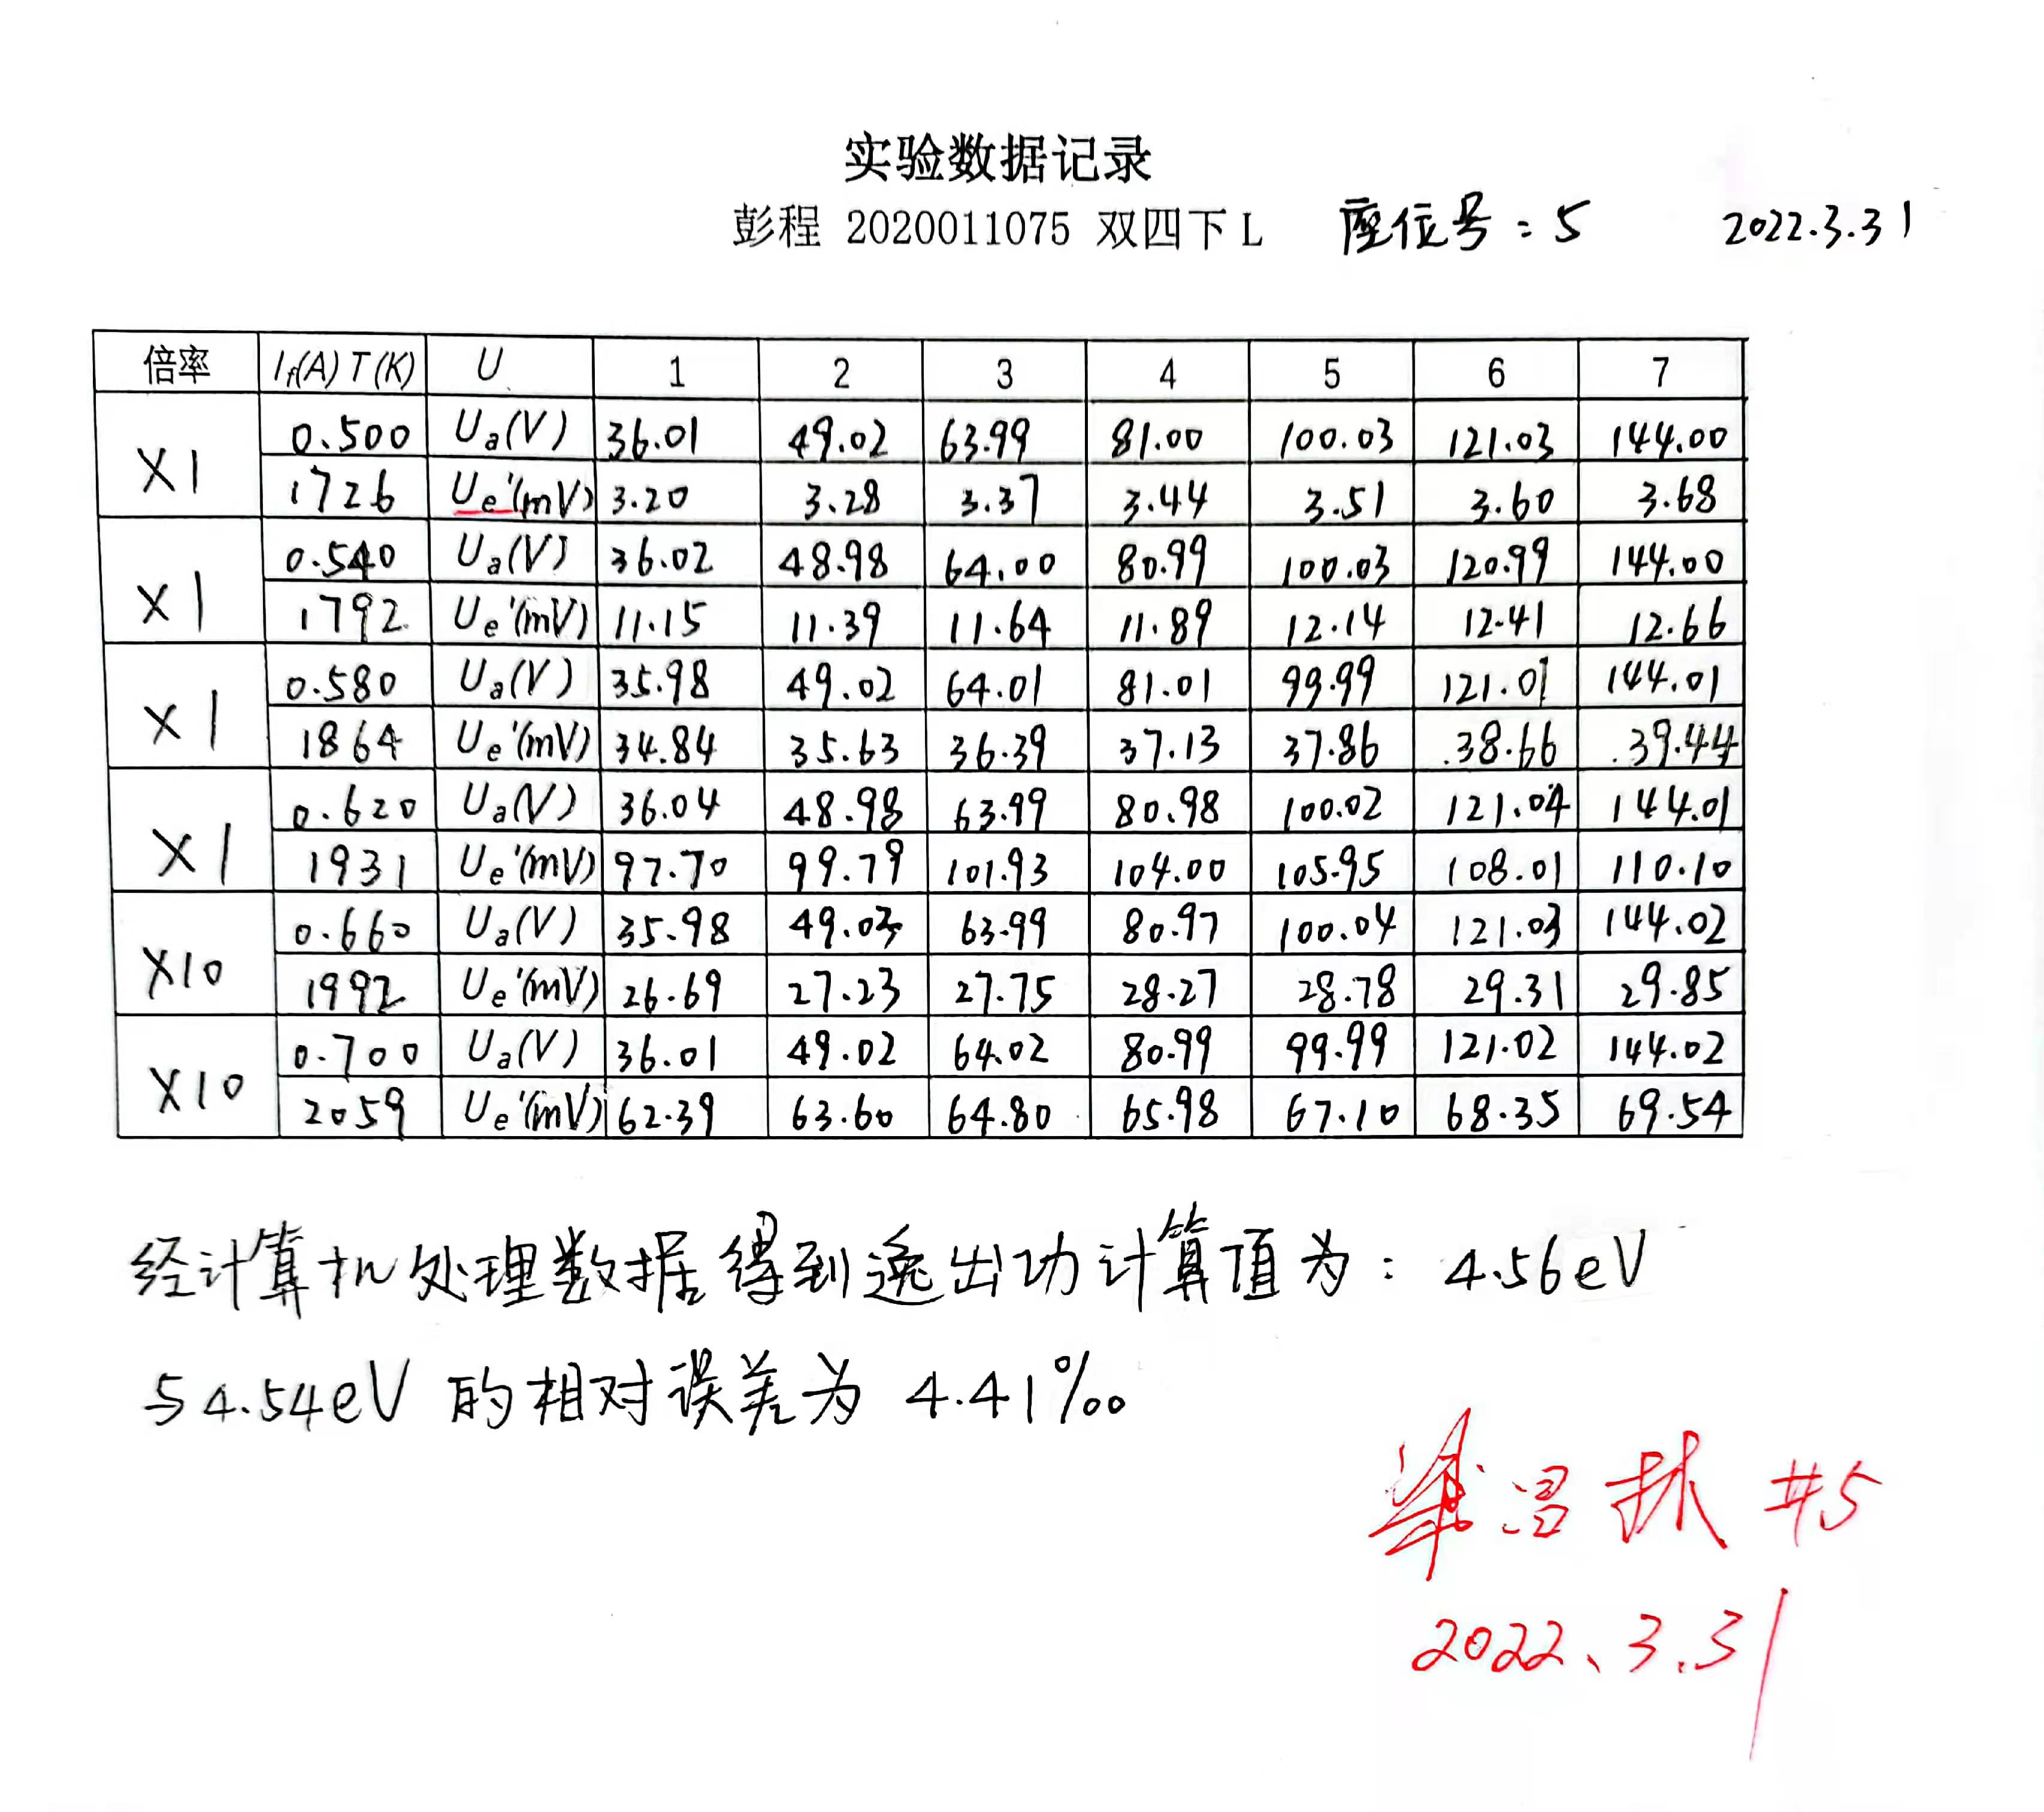
\includegraphics[scale=0.13]{数据.jpg}
\end{figure}

\begin{figure}[H]
  \centering
  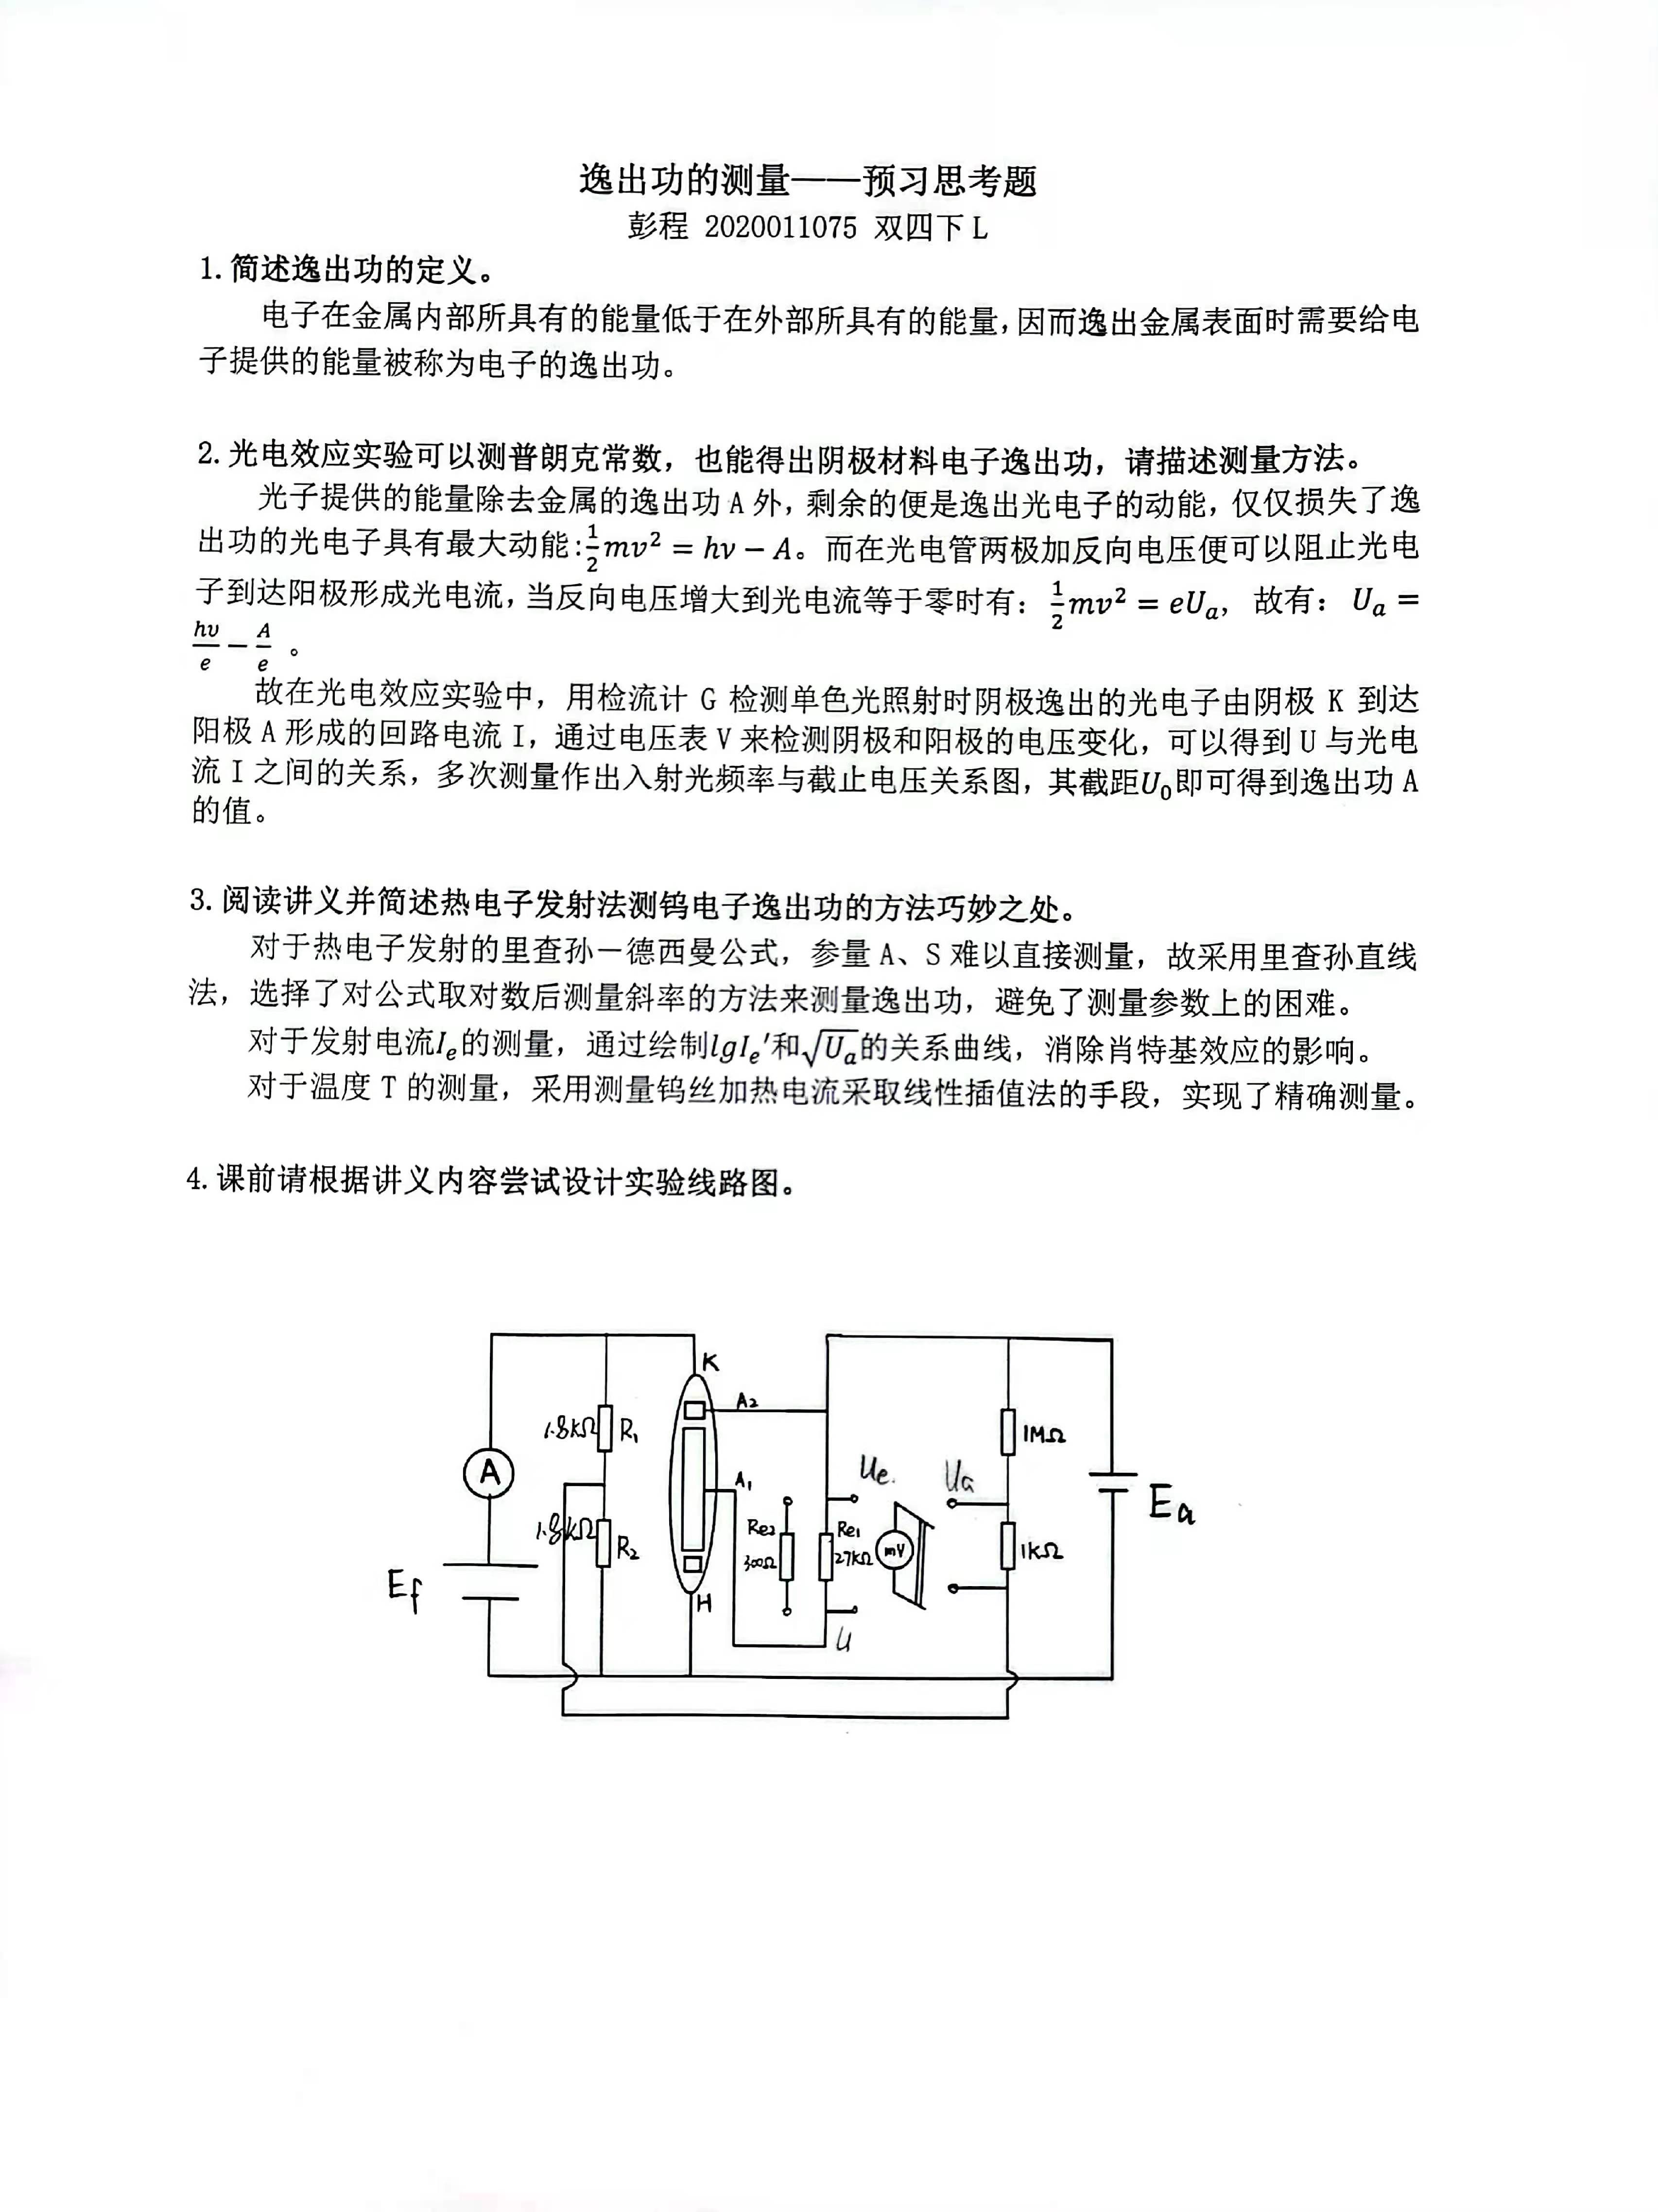
\includegraphics[scale=0.15]{预习.jpg}
\end{figure}

\end{document}